\documentclass[12pt]{report}
\usepackage{graphicx}
\usepackage[utf8]{vietnam}
\usepackage[left=3cm, right=3cm, top=3cm, bottom =3cm]{geometry}
\usepackage{pdfpages}
\usepackage{fancyhdr}
\usepackage{hyperref}
\usepackage{etoolbox}
\usepackage{float}
\usepackage{amsmath}

% \setcounter{tocdepth}{4}

% Link color setup
\hypersetup{
	colorlinks = true,
	linkcolor = black,
	citecolor = blue
}

% Change format of page
\pagestyle{fancy}
\fancyhf{}
\fancyhead{}
\fancyfoot{}
\fancyhead[L]{Kỹ thuật lập trình}
\fancyfoot[L]{Nhóm 4 - KSTN-CNTT-K60}
\fancyfoot[R]{\thepage}
\renewcommand{\headrulewidth}{1pt}
\renewcommand{\footrulewidth}{1pt}

\patchcmd{\chapter}{\thispagestyle{plain}}{\thispagestyle{fancy}}{}{}

\renewcommand{\thesection}{\arabic{section}}
\renewcommand{\thesubsection}{\thesection.\arabic{subsection}}
\renewcommand{\thesubsubsection}{\thesubsection.\arabic{subsubsection}}

% format
\usepackage{titlesec}
\usepackage{etoolbox}
\makeatletter
\patchcmd{\ttlh@hang}{\parindent\z@}{\parindent\z@\leavevmode}{}{}
\patchcmd{\ttlh@hang}{\noindent}{}{}{}
\makeatother

\titleformat{\subsection}
{\normalfont\large\bfseries}{\thesubsection}{1em}{}
\titleformat{\subsubsection}
{\normalfont\large\sffamily\bfseries}{\thesubsubsection}{1em}{}

%--------------------------------------------------------------
% 					PYTHON
%--------------------------------------------------------------
% Default fixed font does not support bold face
\DeclareFixedFont{\ttb}{T1}{txtt}{bx}{n}{12} % for bold
\DeclareFixedFont{\ttm}{T1}{txtt}{m}{n}{12}  % for normal

% Custom colors
\usepackage{color}
\definecolor{deepblue}{rgb}{0,0,0.5}
\definecolor{deepred}{rgb}{0.6,0,0}
\definecolor{deepgreen}{rgb}{0,0.5,0}

\usepackage{listings}

% Python style for highlighting
\newcommand\pythonstyle{\lstset{
language=Python,
basicstyle=\sffamily\ttm,
otherkeywords={self},             % Add keywords here
keywordstyle=\sffamily\bfseries\ttb\color{deepblue},
emph={MyClass,__init__},          % Custom highlighting
emphstyle=\sffamily\ttb\color{deepred},    % Custom highlighting style
stringstyle=\sffamily\color{deepgreen},
frame=tb,                         % Any extra options here
showstringspaces=false ,        % 
tabsize = 4
}}

% Python environment
\lstnewenvironment{python}[1][]
{
\pythonstyle
\lstset{#1}
}
{}

% Python for external files
\newcommand\pythonexternal[2][]{{
\pythonstyle
\lstinputlisting[#1]{#2}}}

% Python for inline
\newcommand\pythoninline[1]{{\pythonstyle\lstinline!#1!}}
%----------------------------------------------------------------
% 							END PYTHON
%----------------------------------------------------------------

\begin{document}

\includepdf{title.pdf}

\newpage
\setcounter{page}{1}

\tableofcontents 
\newpage

\section{Khái quát về mạng Bayes}
Là một đồ thị có hướng phi chu trình mà trong đó:
\begin{itemize}
\item Các nút biểu diễn các biến ngẫu nhiên
\item Các cạnh biểu diễn các phụ thuộc xác suất giữa các biến ngẫu nhiên tương ứng
\end{itemize}
Nếu có một cạnh từ nút $A$ tới nút $B$, thì $B$ phụ thuộc trực tiếp vào biến $A$, và $A$ được 
gọi là cha của $B$, còn $B$ là con của $A$.
\begin{itemize}
\item Nếu biến được thể hiện bởi một nút được quan sát thì nó được gọi là nút chứng cứ.
Nếu không, nút đó được gọi là nút ẩn.
\item Nếu $X_i$ không có cha, ta nói rằng phân phối xác suất của nó là không có điều kiện. 
\end{itemize}
\begin{figure}[h]
\centering
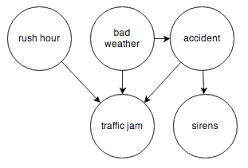
\includegraphics[scale=1]{mang-bayesian.png}
\caption{Một mạng Bayes đơn giản}
\end{figure}

\section{Tính chất của mạng Bayes}
\begin{itemize}
\item Mạng Bayes là một đồ thị định hướng phi chu trình.
\item Về mặt định lượng, các nút được đính kèm một bảng phân phối xác suất phụ 
thuộc vào các nút cha mẹ của nó (CPD - conditional probability distribution) (nếu có).
\item Nếu với mỗi biến $X_i$, tập hợp các biến cha được ký hiệu bởi $parents(X_i)$ thì phân
phối có điều kiện đồng thời bởi các biến  đó được thể hiện bởi công thức: 
$$Pr(X_1, ..., X_n) = \prod_{i=1}^n Pr(X_i | parents(X_i))$$
\end{itemize}

\section{Ví dụ}
\begin{figure}[h]
\centering
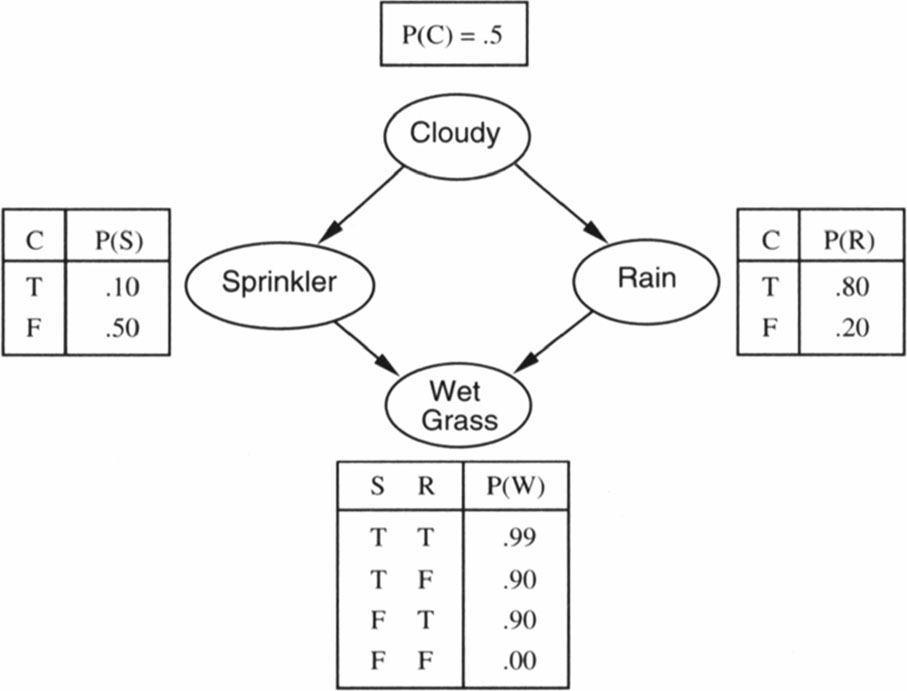
\includegraphics[width=11cm]{vi-du.jpg}
\caption{Ví dụ về mạng Bayes}
\end{figure}

\begin{align*}
P(C, S, R, W)&=P(W| S, R, C) P(S | R, C) P(R | C) P(C) \\
			&= P(W|S, R) P(S, C) P(R|C) P(C) 
\end{align*}

\begin{align*}
P(R=T|W=T) &= \frac{P(R=T, W=T)}{P(W=T)} 			\\
		   &= \frac{\sum_{S, C} P(R=T, S, C, W=T)}{\sum_{S, R, C} P(W=T, S, R, C)}
\end{align*}

\section{Học mạng Bayes}
\begin{itemize}
\item Công việc xây dựng mạng phức tạp với con người. Do vậy phải thực hiện công việc học tập  cấu trúc và tham số mạng từ dữ liệu.
\item Vấn đề này được gọi là BN learning (học mạng Bayes), có thể được mô tả như sau:
\begin{itemize}
\item Cho bộ dữ liệu và thông tin liên quan. 
\item Tìm cấu trúc của mô hình mạng Bayes đồng thời xác định định lượng
	các thông số của nó.
\end{itemize}
\item Độ tốt của giải thuật learning: Đưa ra hàm tính điểm tương ứng với mạng Bayes tìm được.
\end{itemize}

\subsection{Sơ lược về Học cấu trúc}
\begin{itemize}
\item Giả sử dữ liệu được sinh ra từ một mạng Bayes và tất cả các biến là quan sát được, việc tối ưu hóa dựa trên phương pháp tìm kiếm có thể được dung để tìm hiểu cấu trúc mạng. 
\item Một cách tiếp cận khác là sử dụng chiến lược tìm kiếm địa phương để tìm một cấu trúc tại địa phương, tối ưu hóa điểm số của nó một cách cục bộ, rồi tìm cách mở rộng địa phương ra hướng về toàn cục.
\end{itemize}
\subsection{Sơ lược về Học tham số}
\begin{itemize}
\item Đối với mỗi biến $X$, cần chỉ ra phân bố xác suất $X$ theo điều kiện thông tin từ các cha của $X$.
\item Các phân bố có điều kiện này bao gồm các tham số chưa biết, phải được ước lượng từ dữ liệu.
\item Một trong những cách ước lượng là phương pháp MLE, và EM
\end{itemize}
\subsection{Bốn trường hợp BN learning}
\begin{itemize}
\item Maximum – likelihood estimation
\item EM (or gradient ascent), MCMC
\item Search through model space
\item EM + search through model space
\end{itemize}

\begin{table}[h]
\caption{Bốn trường hợp của học mạng Bayes}
\centering
\begin{tabular}{|l|l|l|l|}
\hline
Case & BN structure & Observability & Proposed learning method \\
\hline 
1 & Known & Full & Maximum-likelihood estimation			\\
2 & Known & Partial & EM (or gradient ascent), MCMC \\
3 & Unknown & Full & Search through model space \\
4 & Unknown & Partial & EM + search through model space \\
\hline
\end{tabular}
\end{table}
\subsubsection{Maximum likelihood estimation (MLE)}
\begin{itemize}
\item Sử dụng khi biết cấu trúc mạng và có thể quan sát toàn bộ dữ liệu
\item Còn được gọi là phương pháp hợp lý cực đại
\item Tập dữ liệu gồm $m$ trường hợp độc lập nhau.
\item Cho tập dữ liệu huấn luyện: $\Sigma = \{x_1, x_2, ..., x_m\}$, trong đó $x_i = (x_{i,1}, ..., x_{i,n})$
Và tập tham số $\Theta = (\theta_1, ..., \theta_n)$, trong đó $\theta_j$ là vector tham số của biến ngẫu nhiên $X_j$.
\item Hàm tính điểm cho kết quả của tham số là hàm likelihood:
$$log L(\Theta|\Sigma) = \sum_{i = 0} ^ m \sum_{j = 0} ^ n log P(x_{i,j} | \pi_j, \theta_j)$$
\end{itemize}

\subsubsection{EM (or gradient ascent), MCMC}
\begin{itemize}
\item Cho trước cấu trúc mạng, nhưng chỉ quan sát được một phần
\item Sử dụng tối đa hóa kỳ vọng (expectation maximization)
\item Thuật toán này thực tế là tìm kiếm một MLE địa phương của các tham số.
\item MCMC (Markov chain Monte Carlo) là một cách tiếp cận khác đã được sử dụng để ước lượng tham số của mô hình BN. 
\end{itemize}

\subsubsection{Search through Model Space}
\begin{itemize}
\item Đây là trường hợp không biết cấu trúc mạng nhưng quan sát được toàn bộ.
\item Mục tiêu là tìm được một cấu trúc mạng có thể giải thích tốt nhất mối quan hệ giữa các biến.
\item Vấn đề tìm kiếm đòi hỏi một hàm tính điểm và một chiến lược tìm kiếm
\item Đây là một vấn đề NP – khó vì để duyệt toàn bộ cấu trúc định hướng phi chu trình (DAG) đòi hỏi thời gian cấp siêu lũy thừa đối với số biến.
\item Một cách tiếp cận được đề xuất là xây dựng mạng Naïve BN.
\end{itemize}

\textbf{Naïve BN}
\begin{itemize}
\item[-] Những biến độc lập được nhóm vào một 
Class, trong đó có một nút cha duy nhất, các 
nút còn lại đều là con của nó.
\item[-] Sử dụng mạng Naïve BN trong thực nghiệm 
Cho thấy kết quả đem lại khá khả quan trong
Nhiều trường hợp thực tế.
\end{itemize}

\begin{figure}[h]
\centering
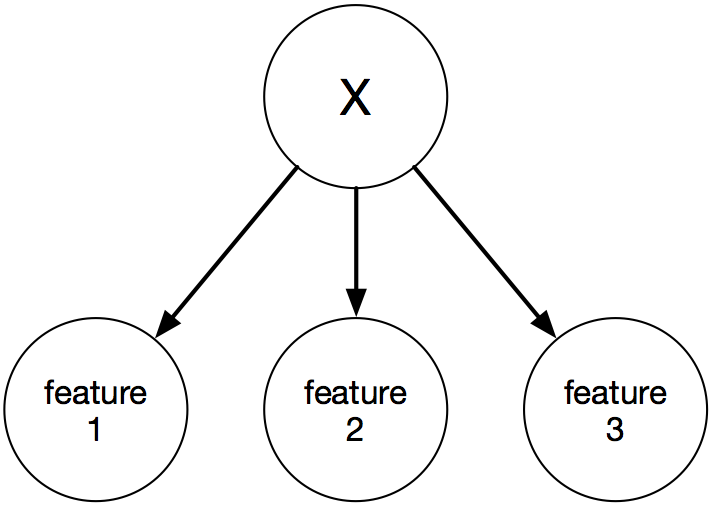
\includegraphics[width=10cm]{naive-bayes.png}
\caption{Naïve BN}
\end{figure}

\subsubsection{EM + search through model space }
\begin{itemize}
\item Kết hợp hai phương pháp xây dựng cấu trúc lẫn tham số trong trường hợp có ít thông tin nhất (không biết cấu trúc mạng, quan sát được một phần)
\item Để có thể sử dụng hàm tính điểm trong việc tìm kiếm cấu trúc, ta phải loại bỏ các nút ẩn và các tham số đi kèm nó.
\item Điều này thường là không giải quyết được nên thường sử dụng một phép xấp xỉ tiệm cận gọi là tiêu chuẩn thông tin (BIC) hay mô tả tối thiểu.
\end{itemize}

\textbf{Bayesian information criterian (BIC)}
\begin{itemize}
\item[-] Xem xét hai thông số là thông số likelihood và thông số penalty.
\item[-] Trong đó likelihood đánh giá độ hợp lý tham số, còn penalty đánh giá độ phức tạp của mô hình
\item[-] Hai thông số này cần được cân bằng để có thể đưa ra điểm số tốt cho thuật toán.
\end{itemize}

\section{Học mạng Bayes bằng Python}
Sử dụng thư viện pgmpy để thao tác trên mạng Bayes. 
\subsection{Học tham số}
\begin{itemize}
\item Maximum likelihood estimation: Tính trực tiếp xác suất dựa trên mẫu bằng cách coi tỉ lệ các thành phần trong mẫu như tỉ lệ trong thực tế.
\item Bayesian Parameter Estimation
\begin{itemize}
\item[-] Bdeu
\item[-] K2
\item[-] Dirichlet
\end{itemize}
\end{itemize}

\subsubsection{Maximum likelihood estimation}
\begin{figure*}[h]
\centering
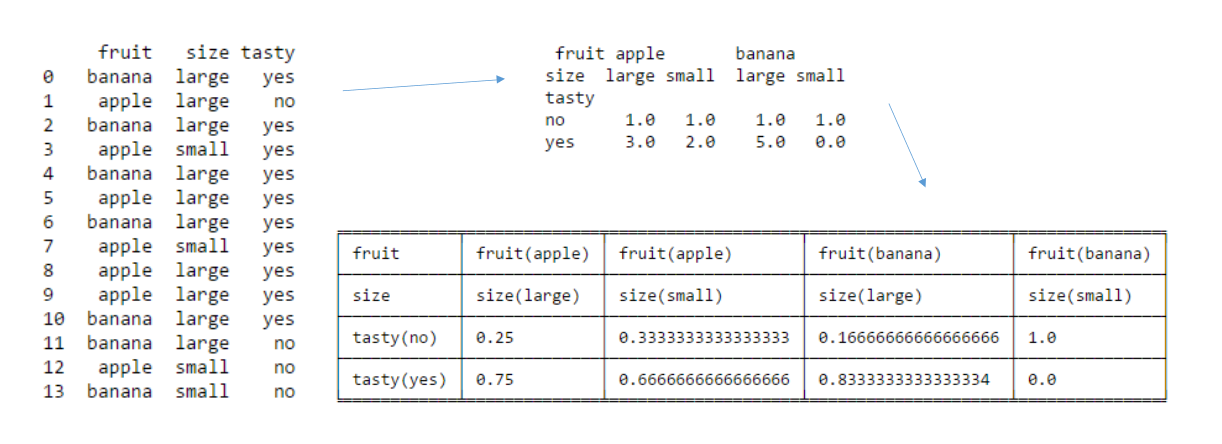
\includegraphics[width=\textwidth]{MLE.png}
\end{figure*}
\subsubsection{Bayesian Parameter Estimation}
\begin{itemize}
\item Diriclet: Đưa ra một pseudo\_counts, là một danh sách các số được dùng để cộng vào mẫu khảo sát của bộ dữ liệu huấn luyện một cách trực tiếp trước khi ước lượng. 

Ví dụ: Pseudo\_counts ta chọn cho bộ dữ liệu là [1,2] 
\item K2: Giống với Diriclet, có điều pseudo\_counts có các phần tử là 1.
\item Bdeu: Cũng dựa trên Diriclet, có điều các phần tử của Pseudo\_counts được tính dựa trên một tham số là equivalent\_sample\_size và khi đó, các phần tử của pseudo\_counts có giá trị là:
$$ \frac{equivalent\_sample\_size}{NodeCardinality * np.prod(ParentsCardinality)}
$$
\end{itemize}

\subsection{Học cấu trúc}
Để học cấu trúc, ta thường có ba hướng: 
\begin{itemize}
\item Một là sử dụng Score-base structure learning
\item Hai là sử dụng Constraint-base structure learning
\item Ba là kết hợp cả hai: Hybird structure learning
\end{itemize}

\subsection{Score – base}
\begin{itemize}
\item Sử dụng các hàm tính điểm để đánh giá độ tốt của cấu trúc mạng. 
\item Các hàm tính điểm trong thư viện pgmpy:
\begin{itemize}
\item BdeuScore
\item K2Score
\item BicScore
\end{itemize}
\item Chiến lược tìm kiếm: Với mạng có rất ít nodes, sử dụng exhaustive search, với mạng có nhiều hơn các node cần phải sử dụng heuristic search. Một trong những giải thuật tìm kiếm đề xuất là HillClimbSearch (thực hiện một tìm kiếm địa phương bằng giải thuật tham lam)
\end{itemize}
\begin{figure*}[h]
\centering
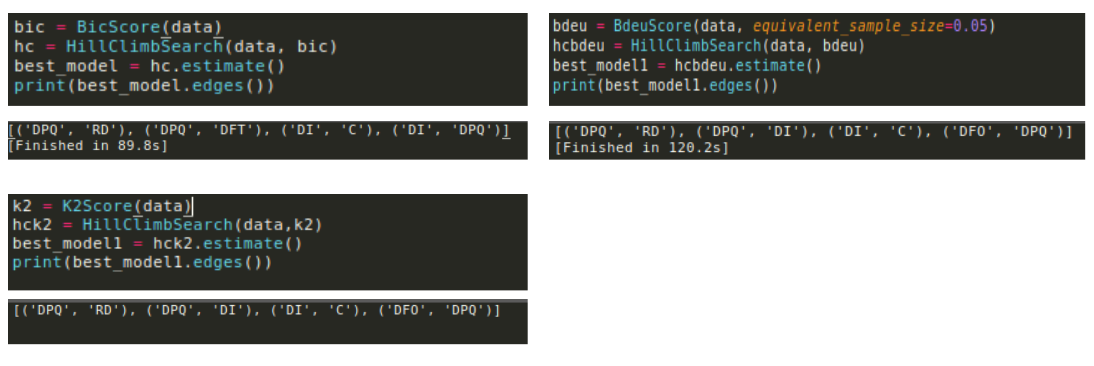
\includegraphics[width=\textwidth]{BIC.png}
\end{figure*}

\subsubsection{Constraint-Base}
Gồm hai bước: 
\begin{itemize}
\item Bước 1: Xác định các node độc lập với nhau.
\begin{itemize}
\item Sử dụng hàm test\_conditional\_independence(X,Y,Zs)
\end{itemize}
\item Bước 2: Xây dựng một mẫu mạng dựa trên các node độc lập đã xác định, gồm 3 bước:
\begin{enumerate}
\item Xây dựng một bộ khung mạng vô hướng bằng hàm estimate\_skeleton()
\item Định hướng các cạnh của mạng để đạt được một mạng có hướng phi chu trình địa phương bằng hàm skeleton\_to\_pdag()
\item Mở rộng mạng địa phương để đạt được mạng toàn cục pdag\_to\_dag()
\end{enumerate}
\end{itemize}
\begin{figure*}[h]
\centering
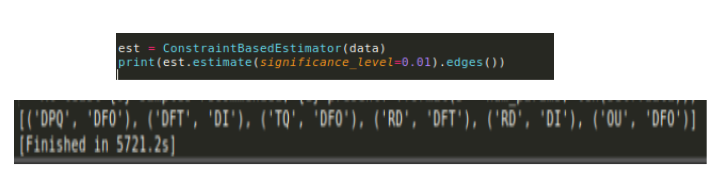
\includegraphics[width=15cm]{constraint-base.png}
\end{figure*}

\subsubsection{Hybrid Structure Learning}
Gồm hai bước:
\begin{itemize}
\item Bước 1: Học một khung đồ thị vô hướng sử dụng thủ tục constraint-based construction MMPC.
\item Bước 2: Định hướng các cạnh sử dụng tối ưu score-based (BdeuScore + modified hill – climbing).
\end{itemize}

\end{document}
